
\section{Σχεσιακό μοντέλο}

\subsection{Πεδία ορισμού}


\begin{tabular}{|p{6cm}|p{8cm}|}
\hline
  Πεδίο Ορισμού & Τύπος                         \\ \hline
  Ακέραιος      & INT                           \\ \hline
  Όνομα         & VARCHAR(40)                   \\ \hline
  Δυαδικό       & ENUMERATED\{Ναι, Όχι\}        \\ \hline
  Εκδηλώσεις    & ENUMERATED\{Εκδήλωση, Μουσική Εκδήλωση, Θεατρική
                  Εκδήλωση, Αθλητική Εκδήλωση\} \\ \hline
  Κείμενο       & VARCHAR(140)                  \\ \hline
  Διεύθυνση     & VARCHAR(35)                   \\ \hline
  Ώρα           & TIME                          \\ \hline
  Ημερομηνία    & DATE                          \\ \hline
  Τηλεφωνο      & VARCHAR(14)                   \\ \hline
  Τιμή          & DEC(2,2)                      \\ \hline
  email         & VARCHAR(30)                   \\ \hline
  pass          & VARCHAR(15)                   \\ \hline
  Αριθμός16     & DEC(16,0)                     \\ \hline
  Αριθμός3      & DEC(3,0)                      \\ \hline
  Εισιτήρια     & VARCHAR(10)                   \\ \hline
\end{tabular}

\subsection{Σχέσεις}

Οι σχέσεις της EventsDB, όπως μεταφέρονται από το μοντέλο οντοτήτων/
συσχετίσεων στην τρίτη κανονική τους μορφή

\begin{tabular}{|p{6cm}|p{8cm}|}
  \hline
  Όνομα Σχέσης          & Εκδήλωση                              \\ \hline
  \multicolumn{2}{|l|}{\textbf{Γνωρίσματα:}}                    \\ \hline
  Όνομα                 & Τύπος                                 \\ \hline
  Κωδικός\_εκδήλωσης     & Ακέραιος                              \\ \hline
  Όνομα                 & Όνομα                                 \\ \hline
  Τύπος                 & Εκδηλώσεις                            \\ \hline
  Κοινό\_που\_απευθύνεται & Όνομα                                 \\ \hline
  Περιγραφή             & Κείμενο                               \\ \hline
  Ημερομηνία            & Ημερομηνία                            \\ \hline
  Ώρα\_έναρξης           & Ώρα                                   \\ \hline
  Κωδικός\_τοπεθεσίας    & Ακέραιος                              \\ \hline
  Κωδικός\_ερμηνευτή     & Ακέραιος                              \\ \hline
  Κωσικός\_διοργανωτή    & Ακέραιος                              \\ \hline
  \multicolumn{2}{|l|}{\textbf{Περιορισμοί Ακεραιότητας:}}      \\ \hline
  Πρωτεύον Κλειδί       & Κωδικός\_εκδήλωσης                     \\ \hline
  Ξένα Κλειδιά          & Κωδικός\_τοποθεσίας -> Τοποθεσία       \\ \cline{2-2}
                        & Κωδικός\_Ερμηνευτή -> Καλητέχνης-Ομάδα \\ \cline{2-2}
                        & Κωδικός\_διοργανώτή -> Διοργανωτής     \\ \hline
\end{tabular}

\begin{tabular}{|p{6cm}|p{8cm}|}
  \hline
  Όνομα Σχέσης            & Μουσική εκδήλωση               \\ \hline
  \multicolumn{2}{|l|}{\textbf{Γνωρίσματα:}}               \\ \hline
  Όνομα                   & Τύπος                          \\ \hline
  Κωδικός\_εκδήλωσης       & Ακέραιος                       \\ \hline
  Ύπαρξη\_θέσεων\_καθημένων & Διαδικό                        \\ \hline
  Είδος                   & Κείμενο                        \\ \hline
  Opening\_act             & Κείμενο                        \\ \hline
  \multicolumn{2}{|l|}{\textbf{Περιορισμοί Ακεραιότητας:}} \\ \hline
  Πρωτεύον Κλειδί         & Κωδικός\_εκδήλωσης              \\ \hline
  Ξένα Κλειδιά            & Κωδικός\_εκδήλωσης -> Εκδήλωση  \\ \hline
\end{tabular}

\begin{tabular}{|p{6cm}|p{8cm}|}
  \hline
  Όνομα Σχέσης      & Θέατρο                               \\ \hline
  \multicolumn{2}{|l|}{\textbf{Γνωρίσματα:}}               \\ \hline
  Όνομα             & Τύπος                                \\ \hline
  Κωδικός\_εκδήλωσης & Ακέραιος                             \\ \hline
  Ύπαρξη\_θέσεων\_VIP & Διαδικό                              \\ \hline
  Διάρκεια          & Ακέραιος                             \\ \hline
  \multicolumn{2}{|l|}{\textbf{Περιορισμοί Ακεραιότητας:}} \\ \hline
  Πρωτεύον Κλειδί   & Κωδικός\_εκδήλωσης                    \\ \hline
  Ξένα Κλειδιά      & Κωδικός\_εκδήλωσης -> Εκδήλωση        \\ \hline
\end{tabular}

\begin{tabular}{|p{6cm}|p{8cm}|}
  \hline
  Όνομα Σχέσης      & Αθλητική\_εκδήλωση                    \\ \hline
  \multicolumn{2}{|l|}{\textbf{Γνωρίσματα:}}               \\ \hline
  Όνομα             & Τύπος                                \\ \hline
  Κωδικός\_εκδήλωσης & Ακέραιος                             \\ \hline
  Ύπαρξη\_θέσεων\_VIP & Διαδικό                              \\ \hline
  Άθλημα            & Κείμενο                              \\ \hline
  \multicolumn{2}{|l|}{\textbf{Περιορισμοί Ακεραιότητας:}} \\ \hline
  Πρωτεύον Κλειδί   & Κωδικός\_εκδήλωσης                    \\ \hline
  Ξένα Κλειδιά      & Κωδικός\_εκδήλωσης -> Εκδήλωση        \\ \hline
\end{tabular}

\begin{tabular}{|p{6cm}|p{8cm}|}
  \hline
  Όνομα Σχέσης      & Εισιτήριο                             \\ \hline
  \multicolumn{2}{|l|}{\textbf{Γνωρίσματα:}}                \\ \hline
  Όνομα             & Τύπος                                 \\ \hline
  Κωδικός\_εκδήλωσης & Ακέραιος                              \\ \hline
  Τύπος\_εισιτηρίου  & Εισιτήρια                             \\ \hline
  Τιμή              & Τιμή                                  \\ \hline
  \multicolumn{2}{|l|}{\textbf{Περιορισμοί Ακεραιότητας:}}  \\ \hline
  Πρωτεύον Κλειδί   & Κωδικός\_εκδήλωσης \& Τύπος\_εισιτηρίου \\ \hline
  Ξένο Κλειδί       & Κωδικός\_εκδήλωσης -> Εκδήλωση         \\ \hline
\end{tabular}


\begin{tabular}{|p{6cm}|p{8cm}|}
  \hline
  Όνομα Σχέσης         & Τοποθεσία                         \\ \hline
  \multicolumn{2}{|l|}{\textbf{Γνωρίσματα:}}               \\ \hline
  Όνομα                & Τύπος                             \\ \hline
  Κωδικός\_τοποθεσίας   & Ακέραιος                          \\ \hline
  Όνομα                & Όνομα                             \\ \hline
  Εσωτερικός\_χώρος     & Δυαδικό                           \\ \hline
  Τηλέφωνο             & Τηλέφωνο                          \\ \hline
  Διεύθυνση            & Διεύθυνση                         \\ \hline
  Ύπαρξη\_υποδομών\_ΑΜΕΑ & Δυαδικό                           \\ \hline
  Τιμή\_μπύρας          & Τιμή                              \\ \hline
  Τιμή\_κρασιού         & Τιμή                              \\ \hline
  Τιμή\_Ποτού           & Τιμή                              \\ \hline
  \multicolumn{2}{|l|}{\textbf{Περιορισμοί Ακεραιότητας:}} \\ \hline
  Πρωτεύον Κλειδί      & Κωδικός\_τοποθεσίας                \\ \hline
\end{tabular}


\begin{tabular}{|p{6cm}|p{8cm}|}
  \hline
  Όνομα Σχέσης      & Καλλιτέχνης-Ομάδα                    \\ \hline
  \multicolumn{2}{|l|}{\textbf{Γνωρίσματα:}}               \\ \hline
  Όνομα             & Τύπος                                \\ \hline
  Κωδικός\_ερμηνευτή & Ακέραιος                             \\ \hline
  Ονοματεπώνυμο     & Όνομα                                \\ \hline
  Καταγωγή          & Όνομα                                \\ \hline
  \multicolumn{2}{|l|}{\textbf{Περιορισμοί Ακεραιότητας:}} \\ \hline
  Πρωτεύον Κλειδί   & Κωδικός\_ερμηνευτή                    \\ \hline
\end{tabular}

\begin{tabular}{|p{6cm}|p{8cm}|}
  \hline
  Όνομα Σχέσης        & Καλλιτέχνης                            \\ \hline
  \multicolumn{2}{|l|}{\textbf{Γνωρίσματα:}}                   \\ \hline
  Όνομα               & Τύπος                                  \\ \hline
  Κωδικός\_ερμηνευτή   & Ακέραιος                               \\ \hline
  Είδος               & Όνομα                                  \\ \hline
  Ημερομηνία\_γέννησης & Ημερομηνία                             \\ \hline
  \multicolumn{2}{|l|}{\textbf{Περιορισμοί Ακεραιότητας:}}     \\ \hline
  Πρωτεύον Κλειδί     & Κωδικός\_ερμηνευτή                      \\ \hline
  Ξένο Κλειδί         & Κωδικός\_ερμηνευτή -> Καλλιτέχνης-Ομάδα \\ \hline
\end{tabular}

\begin{tabular}{|p{6cm}|p{8cm}|}
  \hline
  Όνομα Σχέσης      & Ομάδα                                  \\ \hline
  \multicolumn{2}{|l|}{\textbf{Γνωρίσματα:}}                 \\ \hline
  Όνομα             & Τύπος                                  \\ \hline
  Κωδικός\_ερμηνευτή & Ακέραιος                               \\ \hline
  Όνομα\_υπευθύνου   & Όνομα                                  \\ \hline
  \multicolumn{2}{|l|}{\textbf{Περιορισμοί Ακεραιότητας:}}   \\ \hline
  Πρωτεύον Κλειδί   & Κωδικός\_ερμηνευτή                      \\ \hline
  Ξένο Κλειδί       & Κωδικός\_ερμηνευτή -> Καλλιτέχνης-Ομάδα \\ \hline
\end{tabular}


\begin{tabular}{|p{6cm}|p{8cm}|}
  \hline
  Όνομα Σχέσης    & Φυσικό\_σημείο\_προπώλησης               \\ \hline
  \multicolumn{2}{|l|}{\textbf{Γνωρίσματα:}}               \\ \hline
  Όνομα           & Τύπος                                  \\ \hline
  Κωδικός\_σημείου & Ακέραιος                               \\ \hline
  Όνομα           & Όνομα                                  \\ \hline
  Τηλέφωνο        & Τηλέφωνο                               \\ \hline
  Διεύθυνση       & Διεύθυνση                              \\ \hline
  \multicolumn{2}{|l|}{\textbf{Περιορισμοί Ακεραιότητας:}} \\ \hline
  Πρωτεύον Κλειδί & Κωδικός\_σημείου                        \\ \hline
\end{tabular}

\begin{tabular}{|p{6cm}|p{8cm}|}
  \hline
  Όνομα Σχέσης      & Προπώληση                            \\ \hline
  \multicolumn{2}{|l|}{\textbf{Γνωρίσματα:}}               \\ \hline
  Όνομα             & Τύπος                                \\ \hline
  Κωδικός\_σημείου   & Ακέραιος                             \\ \hline
  Κωδικός\_εκδήλωσης & Ακέραιος                             \\ \hline
  Πρωτεύον Κλειδί   & Κωδικός\_σημείου \& Κωδικός\_εκδήλωσης \\ \hline
  Ξένο Κλειδί       & Κωδικός\_σημείου -> Φυσικό\_σημείο\_προπώλησης
                                                           \\ \hline
                    & Κωδικός\_εκδήλωσης -> Εκδήλωση        \\ \hline
\end{tabular}


\begin{tabular}{|p{6cm}|p{8cm}|}
  \hline
  Όνομα Σχέσης             & Διοργανωτής                   \\ \hline
  \multicolumn{2}{|l|}{\textbf{Γνωρίσματα:}}               \\ \hline
  Όνομα                    & Τύπος                         \\ \hline
  Κωδικός\_διοργανωτή       & Ακέραιος                      \\ \hline
  Όνομα\_εταιρίας           & Όνομα                         \\ \hline
  email                    & email                         \\ \hline
  Τηλέφωνο                 & Τηλέφωνο                      \\ \hline
  password                 & pass                          \\ \hline
  \multicolumn{2}{|l|}{\textbf{Περιορισμοί Ακεραιότητας:}} \\ \hline
  Πρωτεύον Κλειδί          & Κωδικός\_διοργανωτή            \\ \hline
\end{tabular}


\begin{tabular}{|p{6cm}|p{8cm}|}
  \hline
  Όνομα Σχέσης    & Χρήστης                                \\ \hline
  \multicolumn{2}{|l|}{\textbf{Γνωρίσματα:}}               \\ \hline
  Όνομα           & Τύπος                                  \\ \hline
  Κωδικός\_χρήστη  & Ακέραιος                               \\ \hline
  Ονοματεπώνυμο   & Όνομα                                  \\ \hline
  email           & email                                  \\ \hline
  password        & pass                                   \\ \hline
  \multicolumn{2}{|l|}{\textbf{Περιορισμοί Ακεραιότητας:}} \\ \hline
  Πρωτεύον Κλειδί & Κωδικός\_χρήστη                         \\ \hline
\end{tabular}


\begin{tabular}{|p{6cm}|p{8cm}|}
  \hline
  Όνομα Σχέσης      & Κάρτα                                \\ \hline
  \multicolumn{2}{|l|}{\textbf{Γνωρίσματα:}}               \\ \hline
  Όνομα             & Τύπος                                \\ \hline
  Αριθμός\_κάρτας    & Αριθμός16                            \\ \hline
  Αριθμός\_ασφαλείας & Αριθμός3                             \\ \hline
  Διεύθυνση         & Διεύθυνση                            \\ \hline
  Κωδικός\_χρήστη    & Ακέραιος                             \\ \hline
  \multicolumn{2}{|l|}{\textbf{Περιορισμοί Ακεραιότητας:}} \\ \hline
  Πρωτεύον Κλειδί   & Αριθμός\_κάρτας                       \\ \hline
  Ξένα Κλειδιά      & Κωδικός\_χρήστη -> Χρήστης            \\ \hline
\end{tabular}

\begin{tabular}{|p{6cm}|p{8cm}|}
  \hline
  Όνομα Σχέσης      & Αγορά                                \\ \hline
  \multicolumn{2}{|l|}{\textbf{Γνωρίσματα:}}               \\ \hline
  Όνομα             & Τύπος                                \\ \hline
  Κωδικός\_εκδήλωσης & Ακέραιος                             \\ \hline
  Κωδικός\_χρήστη    & Ακέραιος                             \\ \hline
  Τύπος\_εισιτηρίου  & Εισιτήρια                            \\ \hline
  \multicolumn{2}{|l|}{\textbf{Περιορισμοί Ακεραιότητας:}} \\ \hline
  Πρωτεύον Κλειδί   & Κωδικός\_χρήστη \& Κωδικός\_εκδήλωσης  \\ \hline
  Ξένα Κλειδιά      & Κωδικός\_χρήστη -> Χρήστης            \\ \hline
                    & Κωδικός\_εκδήλωσης -> Εκδήλωση        \\ \hline
\end{tabular}

\begin{tabular}{|p{6cm}|p{8cm}|}
  \hline
  Όνομα Σχέσης      & Ενδιαφέρον                           \\ \hline
  \multicolumn{2}{|l|}{\textbf{Γνωρίσματα:}}               \\ \hline
  Όνομα             & Τύπος                                \\ \hline
  Κωδικός\_εκδήλωσης & Ακέραιος                             \\ \hline
  Κωδικός\_χρήστη    & Ακέραιος                             \\ \hline
  \multicolumn{2}{|l|}{\textbf{Περιορισμοί Ακεραιότητας:}} \\ \hline
  Πρωτεύον Κλειδί   & Κωδικός\_χρήστη \& Κωδικός\_εκδήλωσης  \\ \hline
  Ξένα Κλειδιά      & Κωδικός\_χρήστη -> Χρήστης            \\ \hline
                    & Κωδικός\_εκδήλωσης -> εκδήλωση        \\ \hline
\end{tabular}



\subsection{Σχεσιακό Σχήμα}

(Δείξτε το σχεσιακό σχήμα για τη βάση. Το σχήμα μπορείτε να το
κατασκευάσετε σε πρόγραμμα της επιλογής σας, ωστόσο θα πρέπει να
ακολουθεί το συμβολισμό του μαθήματος (δηλαδή οι σχέσεις ως κεφαλίδες
πινάκων, τα ξένα κλειδιά ως βέλη μιας κατεύθυνσης, κτλ.))

Παράδειγμα για τη FlightsDB (προσοχή το παράδειγμα δεν είναι πλήρως
αντίστοιχο με το διάγραμμα E/R που δόθηκε παραπάνω – για την εργασία
θα πρέπει να είναι πλήρως αντίστοιχα):

\begin{figure}[H]
  \centering
  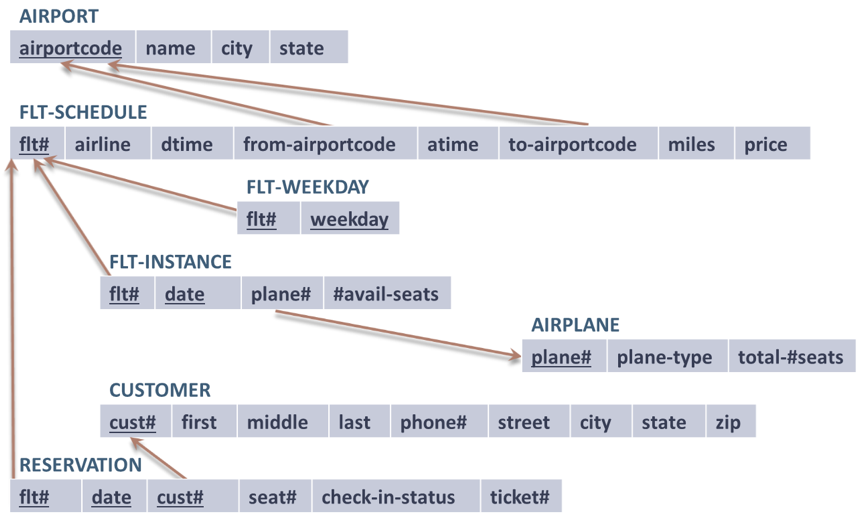
\includegraphics[width=.8\linewidth]{relations.png}
  \caption{Σχεσιακό μοντέλο}
\end{figure}

\subsection{Όψεις}

Παρακάτω παρουσιάζονται κάποιες ενδεικτικές όψεις της βάσης δεδομένων
οι οποίες δίνουν μια πολύ καλή εικόνα για το πως όλες οι σχέσεις
συνδέονται μεταξύ τους. Αρκετές όψεις έχουν πολλές ομοιότητες μεταξύ
τους και γι' αυτόν τον λόγο θα παρουσιάζεται η μία από των μορφών και
ποια η σύνδεση με τις υπόλοιπες όμοιες.

Η κυριότερες όψεις αφορούν την προβολή στοιχείων εκδηλώσεων με διάφορα
κριτήρια. Οποιοσδήποτε συνδυασμός γνωρισμάτων μπορεί να προβληθεί στο
τέλος όμως στην παρακάτω περίπτωση θα προβληθεί μόνο το όνομα της
εκδήλωσης, η ημερομηνία και είτε το όνομα του καταστήματος διεξαγωγής
είτε το όνομα του καλλιτέχνη. Κάποια κριτήρια αναζήτησής εκδηλώσεων
είναι βάση του ονόματος του καταστήματος, όνομα του καλλιτέχνη, ή
συγκεκριμένου τύπου εκδήλωσης.

% >>> insert equation here <<<

Μία εξίσου σημαντική όψη είναι η αναζήτηση μια εκδήλωσης βάση της
ημέρας διεξαγωγής. Είτε για μία συγκεκριμένη ημερομηνία και ώρα είτε
για ένα εύρος.

% >>> insert equation here <<<

Πέρα από τις όψεις των εκδηλώσεων, μία σημαντική όψη αναγκαία για την
ολοκληρωμένη παροχή της υπηρεσίας αγοράς εισιτήριων είναι η προβολή
όλων των χρηστών όπου έχουν πραγματοποιήσει αγορά κάποιου εισιτηρίου
για μια συγκεκριμένη εκδήλωση. Αυτή η όψη θα είναι διαθέσιμη μόνο στον
χρήστη Διοργανωτής ο οποίος συσχετίζεται με την εκάστοτε εκδήλωση.

% >>> insert equation here <<<

Τέλος, μία ακόμα χρήσιμη όψη αφορά τον χρήστη Εγγεγραμμένος Χρήστης ο
οποίος θα θελήσει να προβάλει όλες τις αποθηκευμένες εκδηλώσεις όπου
έχει εκδηλώσει ενδιαφέρων.

% >>> insert equation here <<<


%%% Local Variables:
%%% mode: latex
%%% TeX-master: "main"
%%% End:
